\documentclass[twoside]{book}

% Packages required by doxygen
\usepackage{fixltx2e}
\usepackage{calc}
\usepackage{doxygen}
\usepackage[export]{adjustbox} % also loads graphicx
\usepackage{graphicx}
\usepackage[utf8]{inputenc}
\usepackage{makeidx}
\usepackage{multicol}
\usepackage{multirow}
\PassOptionsToPackage{warn}{textcomp}
\usepackage{textcomp}
\usepackage[nointegrals]{wasysym}
\usepackage[table]{xcolor}

% Font selection
\usepackage[T1]{fontenc}
\usepackage[scaled=.90]{helvet}
\usepackage{courier}
\usepackage{amssymb}
\usepackage{sectsty}
\renewcommand{\familydefault}{\sfdefault}
\allsectionsfont{%
  \fontseries{bc}\selectfont%
  \color{darkgray}%
}
\renewcommand{\DoxyLabelFont}{%
  \fontseries{bc}\selectfont%
  \color{darkgray}%
}
\newcommand{\+}{\discretionary{\mbox{\scriptsize$\hookleftarrow$}}{}{}}

% Page & text layout
\usepackage{geometry}
\geometry{%
  a4paper,%
  top=2.5cm,%
  bottom=2.5cm,%
  left=2.5cm,%
  right=2.5cm%
}
\tolerance=750
\hfuzz=15pt
\hbadness=750
\setlength{\emergencystretch}{15pt}
\setlength{\parindent}{0cm}
\setlength{\parskip}{3ex plus 2ex minus 2ex}
\makeatletter
\renewcommand{\paragraph}{%
  \@startsection{paragraph}{4}{0ex}{-1.0ex}{1.0ex}{%
    \normalfont\normalsize\bfseries\SS@parafont%
  }%
}
\renewcommand{\subparagraph}{%
  \@startsection{subparagraph}{5}{0ex}{-1.0ex}{1.0ex}{%
    \normalfont\normalsize\bfseries\SS@subparafont%
  }%
}
\makeatother

% Headers & footers
\usepackage{fancyhdr}
\pagestyle{fancyplain}
\fancyhead[LE]{\fancyplain{}{\bfseries\thepage}}
\fancyhead[CE]{\fancyplain{}{}}
\fancyhead[RE]{\fancyplain{}{\bfseries\leftmark}}
\fancyhead[LO]{\fancyplain{}{\bfseries\rightmark}}
\fancyhead[CO]{\fancyplain{}{}}
\fancyhead[RO]{\fancyplain{}{\bfseries\thepage}}
\fancyfoot[LE]{\fancyplain{}{}}
\fancyfoot[CE]{\fancyplain{}{}}
\fancyfoot[RE]{\fancyplain{}{\bfseries\scriptsize Generated by Doxygen }}
\fancyfoot[LO]{\fancyplain{}{\bfseries\scriptsize Generated by Doxygen }}
\fancyfoot[CO]{\fancyplain{}{}}
\fancyfoot[RO]{\fancyplain{}{}}
\renewcommand{\footrulewidth}{0.4pt}
\renewcommand{\chaptermark}[1]{%
  \markboth{#1}{}%
}
\renewcommand{\sectionmark}[1]{%
  \markright{\thesection\ #1}%
}

% Indices & bibliography
\usepackage{natbib}
\usepackage[titles]{tocloft}
\setcounter{tocdepth}{3}
\setcounter{secnumdepth}{5}
\makeindex

% Hyperlinks (required, but should be loaded last)
\usepackage{ifpdf}
\ifpdf
  \usepackage[pdftex,pagebackref=true]{hyperref}
\else
  \usepackage[ps2pdf,pagebackref=true]{hyperref}
\fi
\hypersetup{%
  colorlinks=true,%
  linkcolor=blue,%
  citecolor=blue,%
  unicode%
}

% Custom commands
\newcommand{\clearemptydoublepage}{%
  \newpage{\pagestyle{empty}\cleardoublepage}%
}

\usepackage{caption}
\captionsetup{labelsep=space,justification=centering,font={bf},singlelinecheck=off,skip=4pt,position=top}

%===== C O N T E N T S =====

\begin{document}

% Titlepage & ToC
\hypersetup{pageanchor=false,
             bookmarksnumbered=true,
             pdfencoding=unicode
            }
\pagenumbering{roman}
\begin{titlepage}
\vspace*{7cm}
\begin{center}%
{\Large B\+O\+I\+D+\+E\+OS Token-\/staking contract \\[1ex]\large 0.\+1 }\\
\vspace*{1cm}
{\large Generated by Doxygen 1.8.11}\\
\end{center}
\end{titlepage}
\clearemptydoublepage
\tableofcontents
\clearemptydoublepage
\pagenumbering{arabic}
\hypersetup{pageanchor=true}

%--- Begin generated contents ---
\chapter{Action -\/ `\{\{ addbonus \}\}`}
\label{md_src_boidtoken.addbonus_rc}
\hypertarget{md_src_boidtoken.addbonus_rc}{}
This Contract is legally binding and can be used in the event of a dispute. Disputes shall be settled through the standard arbitration process established by E\+O\+S.\+IO.

\subsubsection*{Description}

The {\ttfamily \{\{ addbonus \}\}} action...

I\+N\+T\+E\+NT\+: \+The intent of {\ttfamily \{\{ addbonus \}\}} is to allow an E\+OS account to add additional B\+O\+ID Tokens to the total payout bonus available for the current weekly payout. This most usually will come from the overflow account, but could come from elsewhere. Adding to the payout bonus is always at the sole discretion of the contract owner.

T\+E\+RM\+: \+This action lasts for the duration of the processing of the contract.

\subsubsection*{Inputs and Input Types}

The {\ttfamily \{\{ addbonus \}\}} action requires the following {\ttfamily inputs} and {\ttfamily input types}\+:

\tabulinesep=1mm
\begin{longtabu} spread 0pt [c]{*3{|X[-1]}|}
\hline
\rowcolor{\tableheadbgcolor}{\bf Action }&{\bf Input }&{\bf Input Type  }\\\cline{1-3}
\endfirsthead
\hline
\endfoot
\hline
\rowcolor{\tableheadbgcolor}{\bf Action }&{\bf Input }&{\bf Input Type  }\\\cline{1-3}
\endhead
{\ttfamily \{\{ addbonus \}\}} &{\ttfamily \{\{ \+\_\+sender\+Var \}\}}~\newline
{\ttfamily \{\{ \+\_\+bonus\+Var \}\}} &{\ttfamily \{\{ name \}\}}~\newline
{\ttfamily \{\{ asset \}\}} \\\cline{1-3}
\end{longtabu}

\chapter{Action -\/ `\{\{ checkrun \}\}`}
\label{md_src_boidtoken.checkrun_rc}
\hypertarget{md_src_boidtoken.checkrun_rc}{}
This Contract is legally binding and can be used in the event of a dispute. Disputes shall be settled through the standard arbitration process established by E\+O\+S.\+IO.

\subsubsection*{Description}

The {\ttfamily \{\{ checkrun \}\}} action...

I\+N\+T\+E\+NT\+: The intent of {\ttfamily \{\{ checkrun \}\}} action is to allow the contract owner to review the outcome of an impending execution of the runpayout action. It does not modify any data in tables or otherwise It simply report on the outcome of the current payout forecast for stakers based on current user stake adoption and bonus settings. Execution is restricted to owner only permissions.

T\+E\+RM\+: This action lasts for the duration of the processing of the contract.

\subsubsection*{Inputs and Input Types}

The {\ttfamily \{\{ checkrun \}\}} action requires the following {\ttfamily inputs} and {\ttfamily input types}\+:

\tabulinesep=1mm
\begin{longtabu} spread 0pt [c]{*3{|X[-1]}|}
\hline
\rowcolor{\tableheadbgcolor}{\bf Action }&{\bf Input }&{\bf Input Type  }\\\cline{1-3}
\endfirsthead
\hline
\endfoot
\hline
\rowcolor{\tableheadbgcolor}{\bf Action }&{\bf Input }&{\bf Input Type  }\\\cline{1-3}
\endhead
{\ttfamily \{\{ checkrun \}\}} &&\\\cline{1-3}
\end{longtabu}

\chapter{Action -\/ `\{\{ claim \}\}`}
\label{md_src_boidtoken.claim_rc}
\hypertarget{md_src_boidtoken.claim_rc}{}
This Contract is legally binding and can be used in the event of a dispute. Disputes shall be settled through the standard arbitration process established by E\+O\+S.\+IO.

\subsubsection*{Description}

The {\ttfamily \{\{ claim \}\}} action...

I\+N\+T\+E\+NT\+: The intent of {\ttfamily \{\{ claim \}\}} is to allow users to move token awards from escrow to the staked token storage in the stakes table and to update the users next period stake amount. The users next payout is based on the additional tokens deposited by the system this action also serves to demark the line when the tokens move under user ownership and no longer subject to forfeiture for early withdrawal from the stake period. User participation is required for this action due to the B\+P-\/imposed timeout for transactions over 250ms, which will not allow a contract-\/driven global claim function to be fully executed when over 100 users have staked to the system.

T\+E\+RM\+: This action lasts for the duration of the processing of the contract.

\subsubsection*{Inputs and Input Types}

The {\ttfamily \{\{ claim \}\}} action requires the following {\ttfamily inputs} and {\ttfamily input types}\+:

\tabulinesep=1mm
\begin{longtabu} spread 0pt [c]{*3{|X[-1]}|}
\hline
\rowcolor{\tableheadbgcolor}{\bf Action }&{\bf Input }&{\bf Input Type  }\\\cline{1-3}
\endfirsthead
\hline
\endfoot
\hline
\rowcolor{\tableheadbgcolor}{\bf Action }&{\bf Input }&{\bf Input Type  }\\\cline{1-3}
\endhead
{\ttfamily \{\{ claim \}\}} &{\ttfamily \{\{ \+\_\+stake\+\_\+account\+Var \}\}} &{\ttfamily \{\{ name \}\}} \\\cline{1-3}
\end{longtabu}

\chapter{Action -\/ `\{\{ create \}\}`}
\label{md_src_boidtoken.create_rc}
\hypertarget{md_src_boidtoken.create_rc}{}
This Contract is legally binding and can be used in the event of a dispute. Disputes shall be settled through the standard arbitration process established by E\+O\+S.\+IO.

\subsubsection*{Description}

The {\ttfamily \{\{ create \}\}} action...

I\+N\+T\+E\+NT\+: The intent of {\ttfamily \{\{ create \}\}} is to action... Original unmodified from E\+O\+S\+IO delivered eosio.\+token contract That Ricardian Contract applies here.

T\+E\+RM\+: \+This action lasts for the duration of the processing of the contract.

\subsubsection*{Inputs and Input Types}

The {\ttfamily \{\{ create \}\}} action requires the following {\ttfamily inputs} and {\ttfamily input types}\+:

\tabulinesep=1mm
\begin{longtabu} spread 0pt [c]{*3{|X[-1]}|}
\hline
\rowcolor{\tableheadbgcolor}{\bf Action }&{\bf Input }&{\bf Input Type  }\\\cline{1-3}
\endfirsthead
\hline
\endfoot
\hline
\rowcolor{\tableheadbgcolor}{\bf Action }&{\bf Input }&{\bf Input Type  }\\\cline{1-3}
\endhead
{\ttfamily \{\{ create \}\}} &{\ttfamily \{\{ \+\_\+sender\+Var \}\}}~\newline
{\ttfamily \{\{ \+\_\+bonus\+Var \}\}} &{\ttfamily \{\{ name \}\}}~\newline
{\ttfamily \{\{ asset \}\}} \\\cline{1-3}
\end{longtabu}

\chapter{Action -\/ `\{\{ initstats \}\}`}
\label{md_src_boidtoken.initstats_rc}
\hypertarget{md_src_boidtoken.initstats_rc}{}
This Contract is legally binding and can be used in the event of a dispute. Disputes shall be settled through the standard arbitration process established by E\+O\+S.\+IO.

\subsubsection*{Description}

The {\ttfamily \{\{ initstats \}\}} action...

I\+N\+T\+E\+NT\+: The intent of {\ttfamily \{\{ initstats \}\}} is initialize the contract by placing \char`\"{}0.\+0000 B\+O\+I\+D\char`\"{} in two fields of the config table, and zeros in the config fields of the same table that track user participation amounts and staked account counts. It is intended to be executed once after the initial deployment of the contract and before executing the running action to enable contract staking functions. It could also serve to reset the contract for use under a different stake table in the event of some sort of unforeseen contract failure. Execution is restricted to owner only permissions.

T\+E\+RM\+: This action lasts for the duration of the processing of the contract.

\subsubsection*{Inputs and Input Types}

The {\ttfamily \{\{ initstats \}\}} action requires the following {\ttfamily inputs} and {\ttfamily input types}\+:

\tabulinesep=1mm
\begin{longtabu} spread 0pt [c]{*3{|X[-1]}|}
\hline
\rowcolor{\tableheadbgcolor}{\bf Action }&{\bf Input }&{\bf Input Type  }\\\cline{1-3}
\endfirsthead
\hline
\endfoot
\hline
\rowcolor{\tableheadbgcolor}{\bf Action }&{\bf Input }&{\bf Input Type  }\\\cline{1-3}
\endhead
{\ttfamily \{\{ initstats \}\}} &&\\\cline{1-3}
\end{longtabu}

\chapter{Action -\/ `\{\{ issue \}\}`}
\label{md_src_boidtoken.issue_rc}
\hypertarget{md_src_boidtoken.issue_rc}{}
This Contract is legally binding and can be used in the event of a dispute. Disputes shall be settled through the standard arbitration process established by E\+O\+S.\+IO.

\subsubsection*{Description}

The {\ttfamily \{\{ issue \}\}} action... Original unmodified from E\+O\+S\+IO delivered eosio.\+token contract That Ricardian Contract applies here

\subsubsection*{Inputs and Input Types}

The {\ttfamily \{\{ issue \}\}} action requires the following {\ttfamily inputs} and {\ttfamily input types}\+:

\tabulinesep=1mm
\begin{longtabu} spread 0pt [c]{*3{|X[-1]}|}
\hline
\rowcolor{\tableheadbgcolor}{\bf Action }&{\bf Input }&{\bf Input Type  }\\\cline{1-3}
\endfirsthead
\hline
\endfoot
\hline
\rowcolor{\tableheadbgcolor}{\bf Action }&{\bf Input }&{\bf Input Type  }\\\cline{1-3}
\endhead
{\ttfamily \{\{ issue \}\}} &{\ttfamily \{\{ to\+Var \}\}}~\newline
{\ttfamily \{\{ quantity\+Var \}\}}~\newline
{\ttfamily \{\{ memo\+Var \}\}} &{\ttfamily \{\{ name \}\}}~\newline
{\ttfamily \{\{ asset \}\}}~\newline
{\ttfamily \{\{ string \}\}} \\\cline{1-3}
\end{longtabu}

\chapter{Smart Contract -\/ `\{\{ boidtoken \}\}`}
\label{md_src_boidtoken_rc}
\hypertarget{md_src_boidtoken_rc}{}
This is an overview of the actions for the {\ttfamily \{\{ boidtoken \}\}} smart contract. This Contract is legally binding and can be used in the event of a dispute. Disputes shall be settled through the standard arbitration process established by E\+O\+S.\+IO.

\subsubsection*{Description}

The {\ttfamily \{\{ boidtoken \}\}} C\+O\+N\+T\+R\+A\+CT F\+OR B\+O\+ID T\+O\+K\+E\+N/\+S\+T\+A\+K\+I\+NG C\+O\+N\+T\+R\+A\+CT

O\+V\+E\+R\+A\+LL F\+U\+N\+C\+T\+I\+O\+N \+: This contract is a upgrade/replacement for the original ednazztokens contract which was deployed on Jun-\/19-\/2018, 08\+:29\+:53 AM in block \#1,538,253 by transaction \#\+: 566736553519b432d02074ab0a3b6523dd6b9a394a66bb26c9479b63f5a33537 and deployed by the ednazztokens account.

Unless otherwise explicitly noted here, this contract does not modify or alter that original contract in either intent or function. Original unmodified actions are listed here for ease of reference and are tagged with the notation \mbox{[}original\mbox{]} in their respective file descriptions.

This contract also covers the standard token functions as expressed in the eosio.\+token example contract published by eosio, they are notated below as \mbox{[}original\mbox{]} and are unmodifiedfrom teh eosio delivered original functions in the eosio.\+token contract.

E\+N\+T\+I\+RE A\+G\+R\+E\+E\+M\+E\+NT. This contract contains the entire agreement of the parties, for all described actions, and there are no other promises or conditions in any other agreement whether oral or written concerning the subject matter of this Contract. This contract supersedes any prior written or oral agreements between the parties.

B\+I\+N\+D\+I\+NG C\+O\+N\+S\+T\+I\+T\+U\+T\+I\+ON\+: All the the action described in this contract are subject to the E\+D\+N\+A-\/\+D\+AC constitution as held at https\+://edna.life/constitution , as well a the E\+O\+S\+IO Constitution held at \href{https://github.com/EOS-Mainnet/governance/blob/master/eosio.system/eosio.system-clause-constitution-rc.md}{\tt https\+://github.\+com/\+E\+O\+S-\/\+Mainnet/governance/blob/master/eosio.\+system/eosio.\+system-\/clause-\/constitution-\/rc.\+md} This includes, but is not limited to membership terms and conditions, dispute resolution and severability.

\subsubsection*{Actions, Inputs and Input Types}

The table below contains the {\ttfamily actions}, {\ttfamily inputs} and {\ttfamily input types} for the {\ttfamily \{\{ boidtoken \}\}} contract.

\tabulinesep=1mm
\begin{longtabu} spread 0pt [c]{*3{|X[-1]}|}
\hline
\rowcolor{\tableheadbgcolor}{\bf Action }&{\bf Input }&{\bf Input Type  }\\\cline{1-3}
\endfirsthead
\hline
\endfoot
\hline
\rowcolor{\tableheadbgcolor}{\bf Action }&{\bf Input }&{\bf Input Type  }\\\cline{1-3}
\endhead
{\ttfamily \{\{ create \}\}} &{\ttfamily \{\{ issuer \}\}}~\newline
{\ttfamily \{\{ maximum\+\_\+supply \}\}} &{\ttfamily \{\{ name \}\}}~\newline
{\ttfamily \{\{ asset \}\}} \\\cline{1-3}
{\ttfamily \{\{ issue \}\}} &{\ttfamily \{\{ to \}\}}~\newline
{\ttfamily \{\{ quantity \}\}}~\newline
{\ttfamily \{\{ memo \}\}} &{\ttfamily \{\{ name \}\}}~\newline
{\ttfamily \{\{ asset \}\}}~\newline
{\ttfamily \{\{ string \}\}} \\\cline{1-3}
{\ttfamily \{\{ stake \}\}} &{\ttfamily \{\{ \+\_\+stake\+\_\+account \}\}}~\newline
{\ttfamily \{\{ \+\_\+stake\+\_\+period \}\}}~\newline
{\ttfamily \{\{ \+\_\+staked \}\}} &{\ttfamily \{\{ name \}\}}~\newline
{\ttfamily \{\{ uint8 \}\}}~\newline
{\ttfamily \{\{ asset \}\}} \\\cline{1-3}
{\ttfamily \{\{ unstake \}\}} &{\ttfamily \{\{ \+\_\+stake\+\_\+account \}\}} &{\ttfamily \{\{ name \}\}} \\\cline{1-3}
{\ttfamily \{\{ transfer \}\}} &{\ttfamily \{\{ from \}\}}~\newline
{\ttfamily \{\{ to \}\}}~\newline
{\ttfamily \{\{ quantity \}\}}~\newline
{\ttfamily \{\{ memo \}\}} &{\ttfamily \{\{ name \}\}}~\newline
{\ttfamily \{\{ name \}\}}~\newline
{\ttfamily \{\{ asset \}\}}~\newline
{\ttfamily \{\{ string \}\}} \\\cline{1-3}
{\ttfamily \{\{ setoverflow \}\}} &{\ttfamily \{\{ \+\_\+overflow \}\}} &{\ttfamily \{\{ name \}\}} \\\cline{1-3}
{\ttfamily \{\{ addbonus \}\}} &{\ttfamily \{\{ \+\_\+sender \}\}}~\newline
{\ttfamily \{\{ \+\_\+bonus \}\}} &{\ttfamily \{\{ name \}\}}~\newline
{\ttfamily \{\{ asset \}\}} \\\cline{1-3}
{\ttfamily \{\{ runpayout \}\}} &{\ttfamily \{\{ runpayout \}\}} &{\ttfamily \{\{ runpayout \}\}} \\\cline{1-3}
{\ttfamily \{\{ running \}\}} &{\ttfamily \{\{ on\+\_\+switch \}\}} &{\ttfamily \{\{ uint8 \}\}} \\\cline{1-3}
{\ttfamily \{\{ claim \}\}} &{\ttfamily \{\{ claim \}\}} &{\ttfamily \{\{ claim \}\}} \\\cline{1-3}
{\ttfamily \{\{ checkrun \}\}} &{\ttfamily \{\{ checkrun \}\}} &{\ttfamily \{\{ checkrun \}\}} \\\cline{1-3}
{\ttfamily \{\{ rembonus \}\}} &{\ttfamily \{\{ rembonus \}\}} &{\ttfamily \{\{ rembonus \}\}} \\\cline{1-3}
{\ttfamily \{\{ initstats \}\}} &{\ttfamily \{\{ initstats \}\}} &{\ttfamily \{\{ initstats \}\}} \\\cline{1-3}
\end{longtabu}

\chapter{Hierarchical Index}
\section{Class Hierarchy}
This inheritance list is sorted roughly, but not completely, alphabetically\+:\begin{DoxyCompactList}
\item contract\begin{DoxyCompactList}
\item \contentsline{section}{boidtoken}{\pageref{classboidtoken}}{}
\item \contentsline{section}{testboidpower}{\pageref{classtestboidpower}}{}
\end{DoxyCompactList}
\item \contentsline{section}{boidtoken\+:\+:transfer\+\_\+args}{\pageref{structboidtoken_1_1transfer__args}}{}
\end{DoxyCompactList}

\chapter{Class Index}
\section{Class List}
Here are the classes, structs, unions and interfaces with brief descriptions\+:\begin{DoxyCompactList}
\item\contentsline{section}{\hyperlink{classboidtoken}{boidtoken} }{\pageref{classboidtoken}}{}
\item\contentsline{section}{\hyperlink{classtestboidpower}{testboidpower} }{\pageref{classtestboidpower}}{}
\item\contentsline{section}{\hyperlink{structboidtoken_1_1transfer__args}{boidtoken\+::transfer\+\_\+args} }{\pageref{structboidtoken_1_1transfer__args}}{}
\end{DoxyCompactList}

\chapter{File Index}
\section{File List}
Here is a list of all documented files with brief descriptions\+:\begin{DoxyCompactList}
\item\contentsline{section}{src/\hyperlink{boidtoken_8cpp}{boidtoken.\+cpp} }{\pageref{boidtoken_8cpp}}{}
\item\contentsline{section}{src/\hyperlink{boidtoken_8hpp}{boidtoken.\+hpp} }{\pageref{boidtoken_8hpp}}{}
\item\contentsline{section}{tests/src/\hyperlink{testboidpower_8cpp}{testboidpower.\+cpp} }{\pageref{testboidpower_8cpp}}{}
\item\contentsline{section}{tests/src/\hyperlink{testboidpower_8hpp}{testboidpower.\+hpp} }{\pageref{testboidpower_8hpp}}{}
\end{DoxyCompactList}

\chapter{Class Documentation}
\hypertarget{classboidtoken}{}\section{boidtoken Class Reference}
\label{classboidtoken}\index{boidtoken@{boidtoken}}


Inheritance diagram for boidtoken\+:
\nopagebreak
\begin{figure}[H]
\begin{center}
\leavevmode
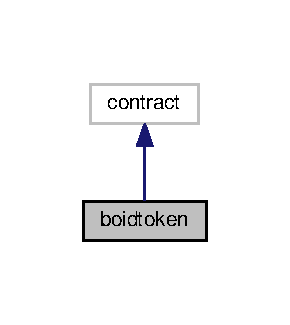
\includegraphics[width=139pt]{classboidtoken__inherit__graph}
\end{center}
\end{figure}


Collaboration diagram for boidtoken\+:
\nopagebreak
\begin{figure}[H]
\begin{center}
\leavevmode
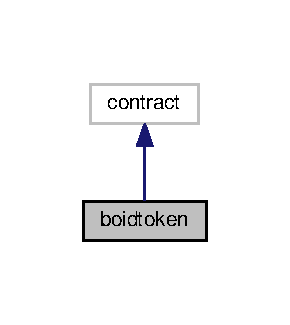
\includegraphics[width=139pt]{classboidtoken__coll__graph}
\end{center}
\end{figure}
\subsection*{Classes}
\begin{DoxyCompactItemize}
\item 
struct \hyperlink{structboidtoken_1_1transfer__args}{transfer\+\_\+args}
\end{DoxyCompactItemize}
\subsection*{Public Member Functions}
\begin{DoxyCompactItemize}
\item 
{\bfseries boidtoken} (account\+\_\+name self)\hypertarget{classboidtoken_a251a26b76724620cd1eb654d32ff4972}{}\label{classboidtoken_a251a26b76724620cd1eb654d32ff4972}

\item 
void \hyperlink{classboidtoken_a09328f276ba96ecb4e2870c6b3433132}{create} (account\+\_\+name issuer, asset maximum\+\_\+supply)
\begin{DoxyCompactList}\small\item\em Add specific token to token-\/staking stats table. \end{DoxyCompactList}\item 
void \hyperlink{classboidtoken_ad4275155b85cfe7932954945f7099cc3}{issue} (account\+\_\+name to, asset quantity, string memo)
\begin{DoxyCompactList}\small\item\em Issuer issues tokens to a specified account. \end{DoxyCompactList}\item 
void \hyperlink{classboidtoken_a81244cb7a5df5ecc52f9ea38d640a763}{transfer} (account\+\_\+name from, account\+\_\+name to, asset quantity, string memo)
\begin{DoxyCompactList}\small\item\em Transfer tokens from one account to another. \end{DoxyCompactList}\item 
void \hyperlink{classboidtoken_ac56437afe05540b627b12e6c7773c793}{setoverflow} (account\+\_\+name \+\_\+overflow)
\begin{DoxyCompactList}\small\item\em Specify overflow account for holding overflow. \end{DoxyCompactList}\item 
void \hyperlink{classboidtoken_af8507dc2ddf06be4b73b5df2def38256}{running} (uint8\+\_\+t on\+\_\+switch)\hypertarget{classboidtoken_af8507dc2ddf06be4b73b5df2def38256}{}\label{classboidtoken_af8507dc2ddf06be4b73b5df2def38256}

\begin{DoxyCompactList}\small\item\em Specify contract run state to contract config table. \end{DoxyCompactList}\item 
void \hyperlink{classboidtoken_af7c0a3fb8818ba690fb053f585026fbb}{stake} (account\+\_\+name \+\_\+stake\+\_\+account, uint8\+\_\+t \+\_\+stake\+\_\+period, asset \+\_\+staked)
\begin{DoxyCompactList}\small\item\em Stake tokens with a specified account. \end{DoxyCompactList}\item 
void \hyperlink{classboidtoken_a25a781212d8a51b13ffa5fa8b899fe8a}{claim} (const account\+\_\+name \+\_\+stake\+\_\+account)
\begin{DoxyCompactList}\small\item\em Claim token-\/staking bonus for specified account. \end{DoxyCompactList}\item 
void \hyperlink{classboidtoken_a53added7a70af2b440581b6f26a57e9f}{unstake} (const account\+\_\+name \+\_\+stake\+\_\+account)
\begin{DoxyCompactList}\small\item\em Unstake tokens from specified account. \end{DoxyCompactList}\item 
void \hyperlink{classboidtoken_ab0897d090230a13a8e5c272bb6ef849d}{checkrun} ()
\begin{DoxyCompactList}\small\item\em Check result of running payout. \end{DoxyCompactList}\item 
void \hyperlink{classboidtoken_ab39151bdead8e592f1d422adf104eebd}{addbonus} (account\+\_\+name \+\_\+sender, asset \+\_\+bonus)\hypertarget{classboidtoken_ab39151bdead8e592f1d422adf104eebd}{}\label{classboidtoken_ab39151bdead8e592f1d422adf104eebd}

\begin{DoxyCompactList}\small\item\em Add bonus to config table. \end{DoxyCompactList}\item 
void \hyperlink{classboidtoken_a828013f2944964600d083ea990684edd}{rembonus} ()\hypertarget{classboidtoken_a828013f2944964600d083ea990684edd}{}\label{classboidtoken_a828013f2944964600d083ea990684edd}

\begin{DoxyCompactList}\small\item\em Transfer unclaimed bonus to overflow account. \end{DoxyCompactList}\item 
void \hyperlink{classboidtoken_a13044fb384103ca5d14029b8aa4fd8bf}{runpayout} ()\hypertarget{classboidtoken_a13044fb384103ca5d14029b8aa4fd8bf}{}\label{classboidtoken_a13044fb384103ca5d14029b8aa4fd8bf}

\begin{DoxyCompactList}\small\item\em Payout staked token bonuses. \end{DoxyCompactList}\item 
void \hyperlink{classboidtoken_ab4f795e1a6d8b363b11c50c50fa00f4b}{initstats} ()\hypertarget{classboidtoken_ab4f795e1a6d8b363b11c50c50fa00f4b}{}\label{classboidtoken_ab4f795e1a6d8b363b11c50c50fa00f4b}

\begin{DoxyCompactList}\small\item\em Initialize config table. \end{DoxyCompactList}\item 
void \hyperlink{classboidtoken_ae5b8eafdb3f1790ef7e601ffb84ff0f7}{reqnewbp} (account\+\_\+name owner)\hypertarget{classboidtoken_ae5b8eafdb3f1790ef7e601ffb84ff0f7}{}\label{classboidtoken_ae5b8eafdb3f1790ef7e601ffb84ff0f7}

\begin{DoxyCompactList}\small\item\em Request new boidpower from boidpower contract. \end{DoxyCompactList}\item 
void \hyperlink{classboidtoken_ae809d2f3f59bd73775d2ac045b0e0134}{setnewbp} (account\+\_\+name bp, account\+\_\+name acct, uint32\+\_\+t boidpower)
\begin{DoxyCompactList}\small\item\em Set new boidpower. \end{DoxyCompactList}\item 
void \hyperlink{classboidtoken_a6e07ac72952b33000b7ab1ff59349d2c}{printstake} (account\+\_\+name owner)
\begin{DoxyCompactList}\small\item\em Print stake of some account. \end{DoxyCompactList}\item 
void \hyperlink{classboidtoken_a611d76eed90fab922d571e04bc2b2fd8}{printbpow} (account\+\_\+name owner)
\begin{DoxyCompactList}\small\item\em Print boidpower of some account. \end{DoxyCompactList}\item 
uint32\+\_\+t \hyperlink{classboidtoken_a58d339c0c3a01a7b046ca250d59bf80f}{get\+\_\+boidpower} (account\+\_\+name owner) const \hypertarget{classboidtoken_a58d339c0c3a01a7b046ca250d59bf80f}{}\label{classboidtoken_a58d339c0c3a01a7b046ca250d59bf80f}

\begin{DoxyCompactList}\small\item\em Get current boidpower of some account in accounts table. \end{DoxyCompactList}\item 
asset \hyperlink{classboidtoken_a6e8a9e31ec29c145bce76662af7e17d5}{get\+\_\+supply} (symbol\+\_\+name sym) const \hypertarget{classboidtoken_a6e8a9e31ec29c145bce76662af7e17d5}{}\label{classboidtoken_a6e8a9e31ec29c145bce76662af7e17d5}

\begin{DoxyCompactList}\small\item\em Get B\+O\+ID token supply. \end{DoxyCompactList}\item 
asset \hyperlink{classboidtoken_af4a97a0262e64dc2d2434cc4a0942ad3}{get\+\_\+balance} (account\+\_\+name owner, symbol\+\_\+name sym) const \hypertarget{classboidtoken_af4a97a0262e64dc2d2434cc4a0942ad3}{}\label{classboidtoken_af4a97a0262e64dc2d2434cc4a0942ad3}

\begin{DoxyCompactList}\small\item\em Get balance of some account for some token in accounts table. \end{DoxyCompactList}\end{DoxyCompactItemize}


\subsection{Member Function Documentation}
\index{boidtoken@{boidtoken}!checkrun@{checkrun}}
\index{checkrun@{checkrun}!boidtoken@{boidtoken}}
\subsubsection[{\texorpdfstring{checkrun()}{checkrun()}}]{\setlength{\rightskip}{0pt plus 5cm}void boidtoken\+::checkrun (
\begin{DoxyParamCaption}
{}
\end{DoxyParamCaption}
)}\hypertarget{classboidtoken_ab0897d090230a13a8e5c272bb6ef849d}{}\label{classboidtoken_ab0897d090230a13a8e5c272bb6ef849d}


Check result of running payout. 

Debugging action \index{boidtoken@{boidtoken}!claim@{claim}}
\index{claim@{claim}!boidtoken@{boidtoken}}
\subsubsection[{\texorpdfstring{claim(const account\+\_\+name \+\_\+stake\+\_\+account)}{claim(const account_name _stake_account)}}]{\setlength{\rightskip}{0pt plus 5cm}void boidtoken\+::claim (
\begin{DoxyParamCaption}
\item[{const account\+\_\+name}]{\+\_\+stake\+\_\+account}
\end{DoxyParamCaption}
)}\hypertarget{classboidtoken_a25a781212d8a51b13ffa5fa8b899fe8a}{}\label{classboidtoken_a25a781212d8a51b13ffa5fa8b899fe8a}


Claim token-\/staking bonus for specified account. 

$\ast$$\ast$$\ast$$\ast$$\ast$$\ast$$\ast$$\ast$$\ast$$\ast$$\ast$$\ast$$\ast$$\ast$$\ast$ D\+A\+I\+LY $\ast$$\ast$$\ast$$\ast$$\ast$$\ast$$\ast$$\ast$$\ast$$\ast$$\ast$$\ast$$\ast$$\ast$$\ast$$\ast$$\ast$$\ast$$\ast$$\ast$$\ast$$\ast$$\ast$$\ast$$\ast$$\ast$$\ast$$\ast$//

$\ast$$\ast$$\ast$$\ast$$\ast$$\ast$$\ast$$\ast$$\ast$$\ast$$\ast$$\ast$$\ast$$\ast$$\ast$ W\+E\+E\+K\+LY $\ast$$\ast$$\ast$$\ast$$\ast$$\ast$$\ast$$\ast$$\ast$$\ast$$\ast$$\ast$$\ast$$\ast$$\ast$$\ast$$\ast$$\ast$$\ast$$\ast$$\ast$$\ast$$\ast$$\ast$$\ast$$\ast$$\ast$$\ast$//

$\ast$$\ast$$\ast$$\ast$$\ast$$\ast$$\ast$$\ast$$\ast$$\ast$$\ast$$\ast$$\ast$$\ast$$\ast$ M\+O\+N\+T\+H\+LY $\ast$$\ast$$\ast$$\ast$$\ast$$\ast$$\ast$$\ast$$\ast$$\ast$$\ast$$\ast$$\ast$$\ast$$\ast$$\ast$$\ast$$\ast$$\ast$$\ast$$\ast$$\ast$$\ast$$\ast$$\ast$$\ast$$\ast$$\ast$//

$\ast$$\ast$$\ast$$\ast$$\ast$$\ast$$\ast$$\ast$$\ast$$\ast$$\ast$$\ast$$\ast$$\ast$$\ast$ Q\+U\+A\+R\+T\+E\+R\+LY $\ast$$\ast$$\ast$$\ast$$\ast$$\ast$$\ast$$\ast$$\ast$$\ast$$\ast$$\ast$$\ast$$\ast$$\ast$$\ast$$\ast$$\ast$$\ast$$\ast$$\ast$$\ast$$\ast$$\ast$$\ast$$\ast$$\ast$$\ast$// \index{boidtoken@{boidtoken}!create@{create}}
\index{create@{create}!boidtoken@{boidtoken}}
\subsubsection[{\texorpdfstring{create(account\+\_\+name issuer, asset maximum\+\_\+supply)}{create(account_name issuer, asset maximum_supply)}}]{\setlength{\rightskip}{0pt plus 5cm}void boidtoken\+::create (
\begin{DoxyParamCaption}
\item[{account\+\_\+name}]{issuer, }
\item[{asset}]{maximum\+\_\+supply}
\end{DoxyParamCaption}
)}\hypertarget{classboidtoken_a09328f276ba96ecb4e2870c6b3433132}{}\label{classboidtoken_a09328f276ba96ecb4e2870c6b3433132}


Add specific token to token-\/staking stats table. 


\begin{DoxyItemize}
\item Set token symbol in table
\item Set token max supply in table
\item Set authorized token issuer in table 
\end{DoxyItemize}\index{boidtoken@{boidtoken}!issue@{issue}}
\index{issue@{issue}!boidtoken@{boidtoken}}
\subsubsection[{\texorpdfstring{issue(account\+\_\+name to, asset quantity, string memo)}{issue(account_name to, asset quantity, string memo)}}]{\setlength{\rightskip}{0pt plus 5cm}void boidtoken\+::issue (
\begin{DoxyParamCaption}
\item[{account\+\_\+name}]{to, }
\item[{asset}]{quantity, }
\item[{string}]{memo}
\end{DoxyParamCaption}
)}\hypertarget{classboidtoken_ad4275155b85cfe7932954945f7099cc3}{}\label{classboidtoken_ad4275155b85cfe7932954945f7099cc3}


Issuer issues tokens to a specified account. 


\begin{DoxyItemize}
\item Specified token must be in stats table
\item Specified quantity must be less than max supply of token to be issued -- Max supply from contract-\/local stats table -- Max supply not necessarily total token supply over entire economy 
\end{DoxyItemize}\index{boidtoken@{boidtoken}!printbpow@{printbpow}}
\index{printbpow@{printbpow}!boidtoken@{boidtoken}}
\subsubsection[{\texorpdfstring{printbpow(account\+\_\+name owner)}{printbpow(account_name owner)}}]{\setlength{\rightskip}{0pt plus 5cm}void boidtoken\+::printbpow (
\begin{DoxyParamCaption}
\item[{account\+\_\+name}]{owner}
\end{DoxyParamCaption}
)}\hypertarget{classboidtoken_a611d76eed90fab922d571e04bc2b2fd8}{}\label{classboidtoken_a611d76eed90fab922d571e04bc2b2fd8}


Print boidpower of some account. 

Debugging action \index{boidtoken@{boidtoken}!printstake@{printstake}}
\index{printstake@{printstake}!boidtoken@{boidtoken}}
\subsubsection[{\texorpdfstring{printstake(account\+\_\+name owner)}{printstake(account_name owner)}}]{\setlength{\rightskip}{0pt plus 5cm}void boidtoken\+::printstake (
\begin{DoxyParamCaption}
\item[{account\+\_\+name}]{owner}
\end{DoxyParamCaption}
)}\hypertarget{classboidtoken_a6e07ac72952b33000b7ab1ff59349d2c}{}\label{classboidtoken_a6e07ac72952b33000b7ab1ff59349d2c}


Print stake of some account. 

Debugging action \index{boidtoken@{boidtoken}!setnewbp@{setnewbp}}
\index{setnewbp@{setnewbp}!boidtoken@{boidtoken}}
\subsubsection[{\texorpdfstring{setnewbp(account\+\_\+name bp, account\+\_\+name acct, uint32\+\_\+t boidpower)}{setnewbp(account_name bp, account_name acct, uint32_t boidpower)}}]{\setlength{\rightskip}{0pt plus 5cm}void boidtoken\+::setnewbp (
\begin{DoxyParamCaption}
\item[{account\+\_\+name}]{bp, }
\item[{account\+\_\+name}]{acct, }
\item[{uint32\+\_\+t}]{boidpower}
\end{DoxyParamCaption}
)}\hypertarget{classboidtoken_ae809d2f3f59bd73775d2ac045b0e0134}{}\label{classboidtoken_ae809d2f3f59bd73775d2ac045b0e0134}


Set new boidpower. 

This is called from boidpower contract \index{boidtoken@{boidtoken}!setoverflow@{setoverflow}}
\index{setoverflow@{setoverflow}!boidtoken@{boidtoken}}
\subsubsection[{\texorpdfstring{setoverflow(account\+\_\+name \+\_\+overflow)}{setoverflow(account_name _overflow)}}]{\setlength{\rightskip}{0pt plus 5cm}void boidtoken\+::setoverflow (
\begin{DoxyParamCaption}
\item[{account\+\_\+name}]{\+\_\+overflow}
\end{DoxyParamCaption}
)}\hypertarget{classboidtoken_ac56437afe05540b627b12e6c7773c793}{}\label{classboidtoken_ac56437afe05540b627b12e6c7773c793}


Specify overflow account for holding overflow. 

Overflow is defined as unclaimed or excess tokens. \index{boidtoken@{boidtoken}!stake@{stake}}
\index{stake@{stake}!boidtoken@{boidtoken}}
\subsubsection[{\texorpdfstring{stake(account\+\_\+name \+\_\+stake\+\_\+account, uint8\+\_\+t \+\_\+stake\+\_\+period, asset \+\_\+staked)}{stake(account_name _stake_account, uint8_t _stake_period, asset _staked)}}]{\setlength{\rightskip}{0pt plus 5cm}void boidtoken\+::stake (
\begin{DoxyParamCaption}
\item[{account\+\_\+name}]{\+\_\+stake\+\_\+account, }
\item[{uint8\+\_\+t}]{\+\_\+stake\+\_\+period, }
\item[{asset}]{\+\_\+staked}
\end{DoxyParamCaption}
)}\hypertarget{classboidtoken_af7c0a3fb8818ba690fb053f585026fbb}{}\label{classboidtoken_af7c0a3fb8818ba690fb053f585026fbb}


Stake tokens with a specified account. 


\begin{DoxyItemize}
\item Add account to stake table or add amount staked to existing account
\item Specify staking period -- Stake period must be valid staking period offered by this contract -- Daily or weekly
\item Specify amount staked -- Token type must be same as type to-\/be-\/staked via this contract 
\end{DoxyItemize}\index{boidtoken@{boidtoken}!transfer@{transfer}}
\index{transfer@{transfer}!boidtoken@{boidtoken}}
\subsubsection[{\texorpdfstring{transfer(account\+\_\+name from, account\+\_\+name to, asset quantity, string memo)}{transfer(account_name from, account_name to, asset quantity, string memo)}}]{\setlength{\rightskip}{0pt plus 5cm}void boidtoken\+::transfer (
\begin{DoxyParamCaption}
\item[{account\+\_\+name}]{from, }
\item[{account\+\_\+name}]{to, }
\item[{asset}]{quantity, }
\item[{string}]{memo}
\end{DoxyParamCaption}
)}\hypertarget{classboidtoken_a81244cb7a5df5ecc52f9ea38d640a763}{}\label{classboidtoken_a81244cb7a5df5ecc52f9ea38d640a763}


Transfer tokens from one account to another. 


\begin{DoxyItemize}
\item Token type must be same as type to-\/be-\/staked via this contract
\item Both accounts of transfer must be valid 
\end{DoxyItemize}\index{boidtoken@{boidtoken}!unstake@{unstake}}
\index{unstake@{unstake}!boidtoken@{boidtoken}}
\subsubsection[{\texorpdfstring{unstake(const account\+\_\+name \+\_\+stake\+\_\+account)}{unstake(const account_name _stake_account)}}]{\setlength{\rightskip}{0pt plus 5cm}void boidtoken\+::unstake (
\begin{DoxyParamCaption}
\item[{const account\+\_\+name}]{\+\_\+stake\+\_\+account}
\end{DoxyParamCaption}
)}\hypertarget{classboidtoken_a53added7a70af2b440581b6f26a57e9f}{}\label{classboidtoken_a53added7a70af2b440581b6f26a57e9f}


Unstake tokens from specified account. 


\begin{DoxyItemize}
\item Return stored escrow to contract account
\item Deduct staked amount from contract config table 
\end{DoxyItemize}

The documentation for this class was generated from the following files\+:\begin{DoxyCompactItemize}
\item 
src/\hyperlink{boidtoken_8hpp}{boidtoken.\+hpp}\item 
src/\hyperlink{boidtoken_8cpp}{boidtoken.\+cpp}\end{DoxyCompactItemize}

\hypertarget{classtestboidpower}{}\section{testboidpower Class Reference}
\label{classtestboidpower}\index{testboidpower@{testboidpower}}


Inheritance diagram for testboidpower\+:
\nopagebreak
\begin{figure}[H]
\begin{center}
\leavevmode
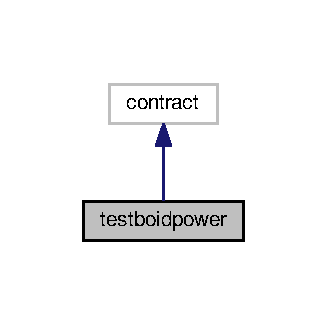
\includegraphics[width=157pt]{classtestboidpower__inherit__graph}
\end{center}
\end{figure}


Collaboration diagram for testboidpower\+:
\nopagebreak
\begin{figure}[H]
\begin{center}
\leavevmode
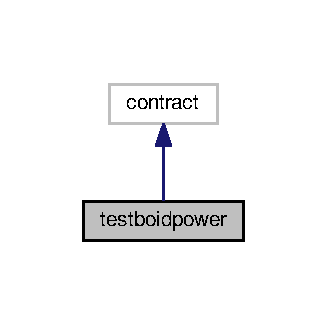
\includegraphics[width=157pt]{classtestboidpower__coll__graph}
\end{center}
\end{figure}
\subsection*{Public Member Functions}
\begin{DoxyCompactItemize}
\item 
{\bfseries testboidpower} (account\+\_\+name self)\hypertarget{classtestboidpower_aa2d01a3deb4873f954c1455b9d698488}{}\label{classtestboidpower_aa2d01a3deb4873f954c1455b9d698488}

\item 
void {\bfseries create} (account\+\_\+name issuer, asset maximum\+\_\+supply)\hypertarget{classtestboidpower_a8a3bf0266a0c39055cc7c48568a19519}{}\label{classtestboidpower_a8a3bf0266a0c39055cc7c48568a19519}

\item 
void {\bfseries insert} (account\+\_\+name user, uint32\+\_\+t boidpower)\hypertarget{classtestboidpower_a6aa85bf9e05658c236c1a63edb07da14}{}\label{classtestboidpower_a6aa85bf9e05658c236c1a63edb07da14}

\item 
void {\bfseries sndnewbp} (account\+\_\+name requester, account\+\_\+name req\+\_\+acct)\hypertarget{classtestboidpower_a742acb44487e0a240cf412d1b93227a3}{}\label{classtestboidpower_a742acb44487e0a240cf412d1b93227a3}

\end{DoxyCompactItemize}


The documentation for this class was generated from the following files\+:\begin{DoxyCompactItemize}
\item 
tests/src/\hyperlink{testboidpower_8hpp}{testboidpower.\+hpp}\item 
tests/src/\hyperlink{testboidpower_8cpp}{testboidpower.\+cpp}\end{DoxyCompactItemize}

\hypertarget{structboidtoken_1_1transfer__args}{}\section{boidtoken\+:\+:transfer\+\_\+args Struct Reference}
\label{structboidtoken_1_1transfer__args}\index{boidtoken\+::transfer\+\_\+args@{boidtoken\+::transfer\+\_\+args}}


Collaboration diagram for boidtoken\+:\+:transfer\+\_\+args\+:
\nopagebreak
\begin{figure}[H]
\begin{center}
\leavevmode
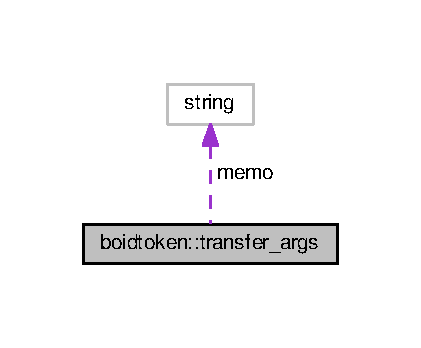
\includegraphics[width=202pt]{structboidtoken_1_1transfer__args__coll__graph}
\end{center}
\end{figure}
\subsection*{Public Attributes}
\begin{DoxyCompactItemize}
\item 
account\+\_\+name {\bfseries from}\hypertarget{structboidtoken_1_1transfer__args_a1fcbad3886dffa5be4229e793f9e5e27}{}\label{structboidtoken_1_1transfer__args_a1fcbad3886dffa5be4229e793f9e5e27}

\item 
account\+\_\+name {\bfseries to}\hypertarget{structboidtoken_1_1transfer__args_a50bbce49431bde906e51c18670c8d055}{}\label{structboidtoken_1_1transfer__args_a50bbce49431bde906e51c18670c8d055}

\item 
asset {\bfseries quantity}\hypertarget{structboidtoken_1_1transfer__args_a71596eabbe596a15a28256a5b2fcabdd}{}\label{structboidtoken_1_1transfer__args_a71596eabbe596a15a28256a5b2fcabdd}

\item 
string {\bfseries memo}\hypertarget{structboidtoken_1_1transfer__args_af285115b0c02cbcc81cac19b75fc1449}{}\label{structboidtoken_1_1transfer__args_af285115b0c02cbcc81cac19b75fc1449}

\end{DoxyCompactItemize}


The documentation for this struct was generated from the following file\+:\begin{DoxyCompactItemize}
\item 
src/\hyperlink{boidtoken_8hpp}{boidtoken.\+hpp}\end{DoxyCompactItemize}

\chapter{File Documentation}
\hypertarget{boidtoken_8cpp}{}\section{src/boidtoken.cpp File Reference}
\label{boidtoken_8cpp}\index{src/boidtoken.\+cpp@{src/boidtoken.\+cpp}}
{\ttfamily \#include \char`\"{}boidtoken.\+hpp\char`\"{}}\\*
{\ttfamily \#include $<$math.\+h$>$}\\*
{\ttfamily \#include $<$inttypes.\+h$>$}\\*
Include dependency graph for boidtoken.\+cpp\+:
\nopagebreak
\begin{figure}[H]
\begin{center}
\leavevmode
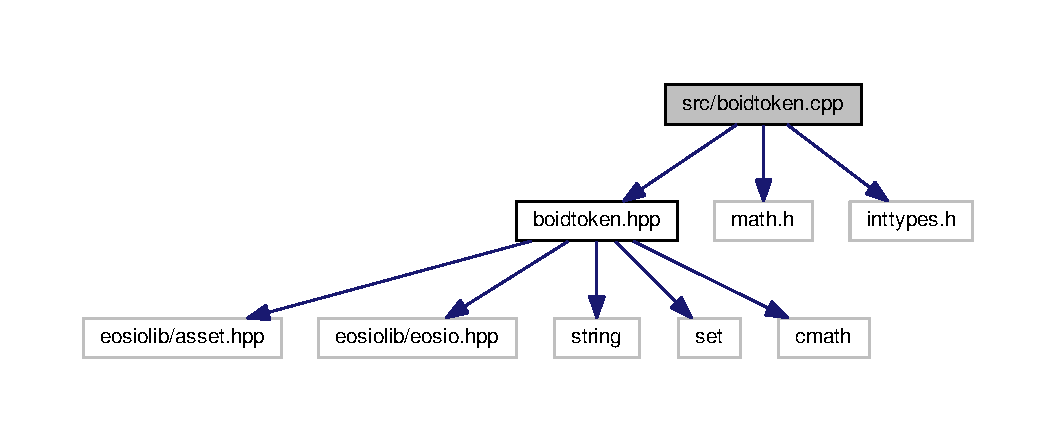
\includegraphics[width=350pt]{boidtoken_8cpp__incl}
\end{center}
\end{figure}


\subsection{Detailed Description}
\begin{DoxyCopyright}{Copyright}
defined in eos/\+L\+I\+C\+E\+N\+S\+E.\+txt 
\end{DoxyCopyright}

\hypertarget{boidtoken_8hpp}{}\section{src/boidtoken.hpp File Reference}
\label{boidtoken_8hpp}\index{src/boidtoken.\+hpp@{src/boidtoken.\+hpp}}
{\ttfamily \#include $<$eosiolib/asset.\+hpp$>$}\\*
{\ttfamily \#include $<$eosiolib/eosio.\+hpp$>$}\\*
{\ttfamily \#include $<$string$>$}\\*
{\ttfamily \#include $<$set$>$}\\*
{\ttfamily \#include $<$cmath$>$}\\*
Include dependency graph for boidtoken.\+hpp\+:
\nopagebreak
\begin{figure}[H]
\begin{center}
\leavevmode
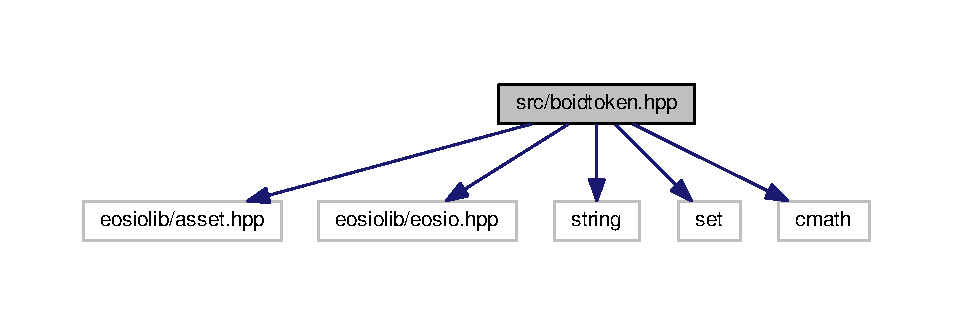
\includegraphics[width=350pt]{boidtoken_8hpp__incl}
\end{center}
\end{figure}
This graph shows which files directly or indirectly include this file\+:
\nopagebreak
\begin{figure}[H]
\begin{center}
\leavevmode
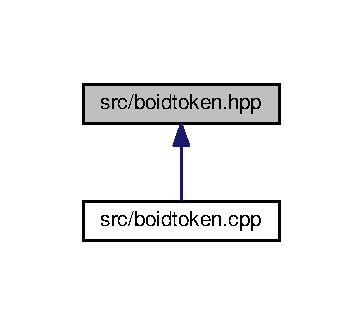
\includegraphics[width=174pt]{boidtoken_8hpp__dep__incl}
\end{center}
\end{figure}
\subsection*{Classes}
\begin{DoxyCompactItemize}
\item 
class \hyperlink{classboidtoken}{boidtoken}
\item 
struct \hyperlink{structboidtoken_1_1transfer__args}{boidtoken\+::transfer\+\_\+args}
\end{DoxyCompactItemize}


\subsection{Detailed Description}
\begin{DoxyCopyright}{Copyright}
defined in eos/\+L\+I\+C\+E\+N\+S\+E.\+txt 
\end{DoxyCopyright}

\hypertarget{testboidpower_8cpp}{}\section{tests/src/testboidpower.cpp File Reference}
\label{testboidpower_8cpp}\index{tests/src/testboidpower.\+cpp@{tests/src/testboidpower.\+cpp}}
{\ttfamily \#include \char`\"{}testboidpower.\+hpp\char`\"{}}\\*
{\ttfamily \#include $<$math.\+h$>$}\\*
Include dependency graph for testboidpower.\+cpp\+:
\nopagebreak
\begin{figure}[H]
\begin{center}
\leavevmode
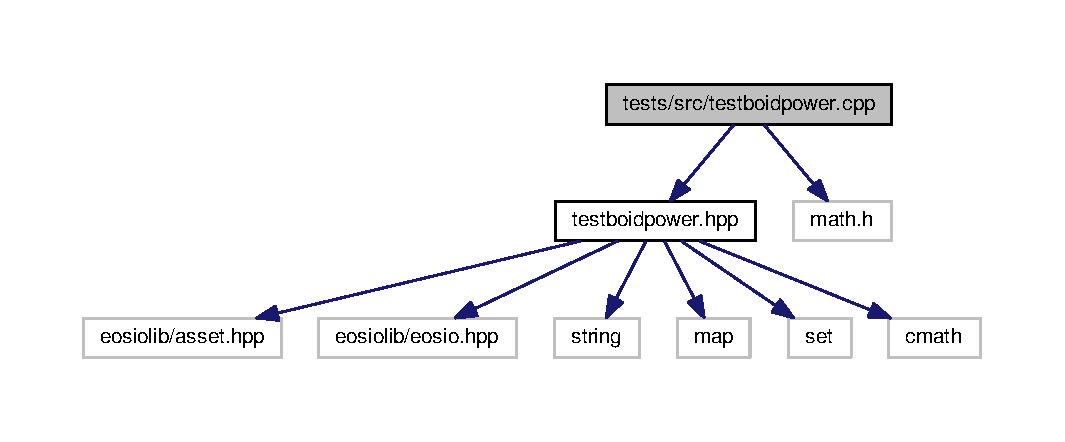
\includegraphics[width=350pt]{testboidpower_8cpp__incl}
\end{center}
\end{figure}


\subsection{Detailed Description}
\begin{DoxyCopyright}{Copyright}
defined in eos/\+L\+I\+C\+E\+N\+S\+E.\+txt 
\end{DoxyCopyright}

\hypertarget{testboidpower_8hpp}{}\section{tests/src/testboidpower.hpp File Reference}
\label{testboidpower_8hpp}\index{tests/src/testboidpower.\+hpp@{tests/src/testboidpower.\+hpp}}
{\ttfamily \#include $<$eosiolib/asset.\+hpp$>$}\\*
{\ttfamily \#include $<$eosiolib/eosio.\+hpp$>$}\\*
{\ttfamily \#include $<$string$>$}\\*
{\ttfamily \#include $<$map$>$}\\*
{\ttfamily \#include $<$set$>$}\\*
{\ttfamily \#include $<$cmath$>$}\\*
Include dependency graph for testboidpower.\+hpp\+:
\nopagebreak
\begin{figure}[H]
\begin{center}
\leavevmode
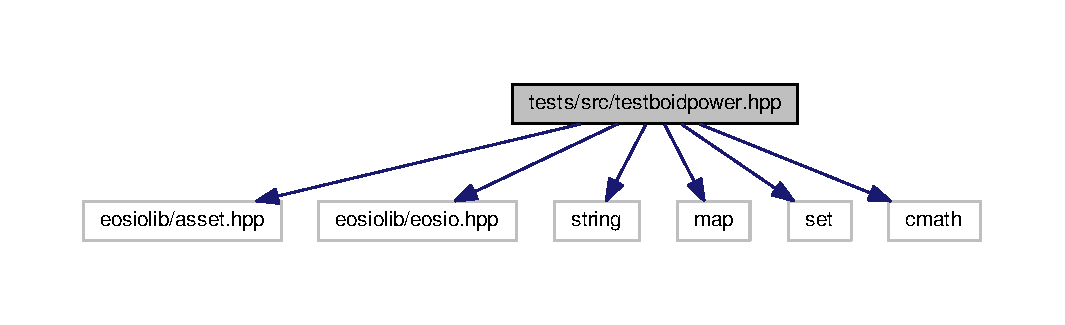
\includegraphics[width=350pt]{testboidpower_8hpp__incl}
\end{center}
\end{figure}
This graph shows which files directly or indirectly include this file\+:
\nopagebreak
\begin{figure}[H]
\begin{center}
\leavevmode
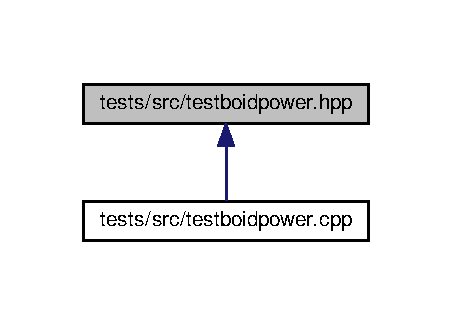
\includegraphics[width=217pt]{testboidpower_8hpp__dep__incl}
\end{center}
\end{figure}
\subsection*{Classes}
\begin{DoxyCompactItemize}
\item 
class \hyperlink{classtestboidpower}{testboidpower}
\end{DoxyCompactItemize}


\subsection{Detailed Description}
\begin{DoxyCopyright}{Copyright}
defined in eos/\+L\+I\+C\+E\+N\+S\+E.\+txt 
\end{DoxyCopyright}

%--- End generated contents ---

% Index
\backmatter
\newpage
\phantomsection
\clearemptydoublepage
\addcontentsline{toc}{chapter}{Index}
\printindex

\end{document}
